\documentclass{beamer}

\usepackage{amsmath}
\usepackage{graphicx}
\usepackage{microtype}

\DisableLigatures{encoding = *, family = *}
\frenchspacing

\mode<beamer>{
  \usetheme{default}
  \usecolortheme{orchid}
  \setbeamertemplate{navigation symbols}{}
}
\mode<handout>{
  \usepackage{pgfpages}
  \pgfpagesuselayout{4 on 1}[a4paper, border shrink=10mm, landscape]
  \usetheme{default}
}


\title{Reading and Interpretation of Alroy's Ten Statistical Commandments}
\subtitle{}
\author{Peter D Smits \inst{1} \inst{2}}
\institute{
  \inst{1}
  School of Biological Sciences\\
  Monash University
  \and
  \inst{2}
  Committee on Evolutionary Biology\\
  University of Chicago
}
\scriptsize{\date{\today}}


\begin{document}
  \mode*
  \begin{frame}
    \titlepage
  \end{frame}



  \begin{frame}
    \frametitle{Background}
    John Alroy is legendary/infamous for getting extremely angry about the use of statistical methods in paleontology (and biology.)
    \\~\\
    Up until about 3 years ago he had a list of 10 statistical commandments on his NCEAS website. 
    Currently he only has an abbreviated version on his website. % put a screengrab of it
    \\~\\
    These are one of the few things I have hanging at my desk.
    \\~\\
    While the content is serious, the presentation is parody.
    The following will be rather \ldots\ sanctimonious.
    \\~\\
    Also, I claim no complete knowledge of what \emph{exactly} I'm discussing.
  \end{frame}



  \begin{frame}
    \frametitle{John Alroy}
    \begin{columns}
      \begin{column}{0.5\textwidth}
          \begin{itemize}
            \item quantitative paleobiologist currently at Macquarie
            \begin{itemize}
              \item diversity curves
              \item PaleoDB
            \end{itemize}
            \item teaches workshop on quantitative methods to prevent future problems \ldots
          \end{itemize}
      \end{column}
      \begin{column}{0.5\textwidth}
      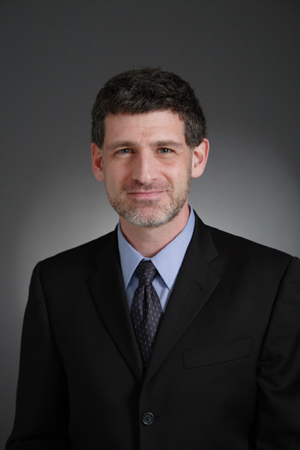
\includegraphics[width = \textwidth, keepaspectratio = true]{dr_john_alroy}
      \end{column}
    \end{columns}
  \end{frame}



  \begin{frame}
    \frametitle{Commandment 1}
    \textbf{Thou shalt log thy data! }
    We live in a multiplicative world, which means our data live in a log world. 
    Always log any data with a lower zero bound, unless there's also an upper bound, 
    in which case that shalt perform a logit transformation. 
    \emph{Log until proven linear, and be holy.}
    % discuss scaling
  \end{frame}
  
  
  \begin{frame}
    \frametitle{Monotonic transform}
    % plot of untransformed and transformed data
    % monotonic transform
  \end{frame}
  
  
  \begin{frame}
    \frametitle{Information and log}
    Imagine we have a device that can give us one of three items at a time: 
    
    A B C
    \\~\\
    Everytime we get something from the device, we receive information and our uncertainty decreases.
    \\~\\
    We can say this device as ``uncertainty 3''
  \end{frame}



  \begin{frame}
    \frametitle{Information and log}
    Now imagine a second device that gives one of two items at a time (uncertainty 2): 
    
    Y Z
    \\~\\
    If we put both devices together, we have six possibilities:
    
    AY AZ BY BZ CY CZ
    \\~\\
    We have 6 instead of 2 (or 5). That is, information is multiplicative not additive. 
    \\~\\
    The easy way to just do this is take the log of the uncertainty of both ``devices.`` Base determines units. Can contiue from here to explain Shannon's entropy (I won't).
    \\~\\
    \(\log 3 + \log 2 = \log 6\)
  \end{frame}
  
  
  
  \begin{frame}
    \frametitle{Commandment 2}
    \textbf{Thou shalt run non-parametric tests! }
    If the parametric and non-parametric tests come out the same, thou hast lost nothing. 
    If they don't, the data are non-normal, the parametric test is wrong, and thou shalt use the non-parametric result. 
    \underline{Spearman}, \underline{Mann-Whitney}, and \underline{Kolmogorov-Smirnov} are the \underline{Holy Trinity} (or Quintinity, or whatever). 
    Worship them!
  \end{frame}
  
  
  
  \begin{frame}
    \frametitle{Non-parametric tests}
    Parametric tests have a number of assumptions (normality).
    Even the basic Pearson's product-momment of correlation (\(r\)) assumes normality.
    \\~\\
    Frequently, these assumptions, either, not tested (homogeneity of variance?)
    or violated (independence).
    \\~\\
    Very rarely in real systems can most tests be applied. 
    Life doesn't always fit in that box.
    \\~\\
    Non-parametric tests avoid (most) of the problems revolving around distributions.
  \end{frame}
  
  
  
  \begin{frame}
    \frametitle{Non-parametric tests}
    Non-parametric statistics, specifically the tests, come in two flavours
    
    \begin{itemize}
      \item distribution free
      \item non-parametric (I love tautologies)
    \end{itemize}
    
    Some examples...
  \end{frame}
  
  
  
  \begin{frame}
    \frametitle{Non-parametric tests}
    
    Spearman rank order coeffecient rho (\(\rho\)) and Kendall's tau (\(\tau\))
    \begin{itemize}
      \item similar to \(r\) but is based on ranks and, thus, distribution free
      \item choice of \(\rho\) or \(\tau\) depends mostly on sample size
    \end{itemize}
    Wilcox signed-rank test and Mann-Whitney U
    \begin{itemize}
      \item similar to \(t\)-test but is based on ranks and is for difference of medians (not means). 
      \item Wilcox is an alternative to paired \(t\)-test
      \item Mann-Whitney is an alternative to two-sample \(t\)-test.
    \end{itemize}
    Kolmogorov-Smirnov test
    \begin{itemize}
      \item Did a sample come from a specific probability distribution (one-sample) or did two samples come from the same probability distribution?
      \item the two-sample is really unique and incredibly useful
    \end{itemize}
  \end{frame}
  
  
  
  \begin{frame}
    \frametitle{Resampling methods}
    Missing from the commandment are resampling methods.
    \\~\\
    Resampling methods (can) have even fewer assumptions than non-parametric methods!
    \\~\\
    In general, you just assume your sample is representative of the population which we do this almost implicitly.
    \\~\\
    Resampling methods are various classes of Monte Carlo methods (randomized) and are generally considered computer intensive.
  \end{frame}
  
  
  
  \begin{frame}
    \frametitle{Resampling methods}
    % need to edit this image
    % left bottom right top
    \centering 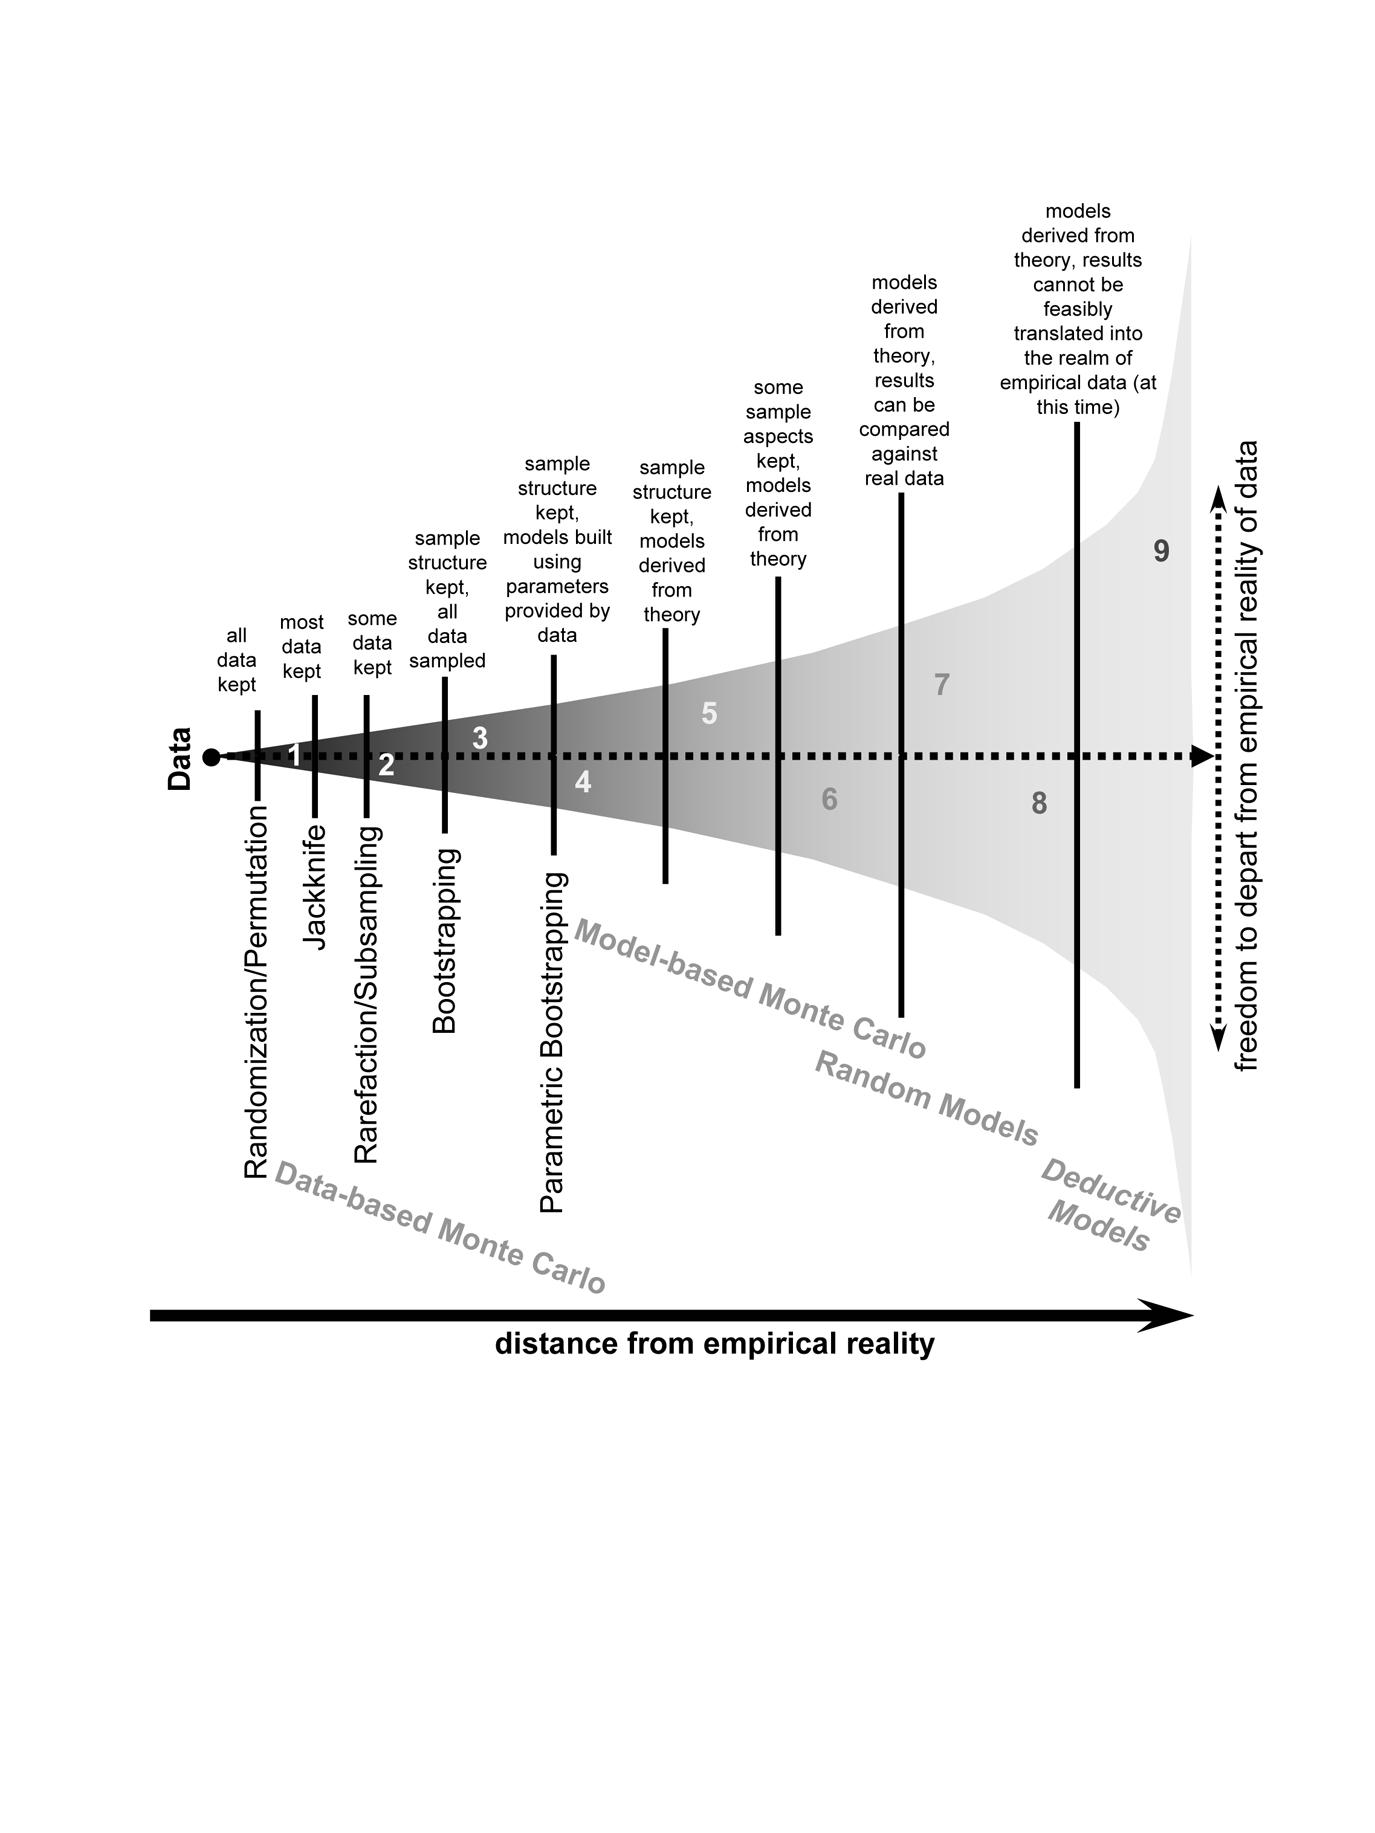
\includegraphics[trim = 0pt 250pt 0pt 75pt, height = 200pt, keepaspectratio = true]{reality}
    
    % need to find a way to put this in bottom right corner
    \footnotesize{from Kowalewski and Novack-Gottshall 2010}
  \end{frame}
  
  
  
  \begin{frame}
    \frametitle{Commandment 3}
    \textbf{Thou shalt disdain p-values! }
    p = 0.05 is a heathen idol, and ANOVAs are for those who have not yet seen the light, still dwelling in the darkness of obsessive frequentist hypothesis testing. 
    Remember, \emph{if thou hast enough data anything will turn significant, no matter how small the difference.} 
    And the ``significance level'' is whatever thou choosest it to be, not what someone tells thee it should be. 
    So, describe data, don't just test data. 
    Don't merely ask \emph{whether} there's a significant difference, ask \emph{what} is the difference, \emph{why} is there a difference, and \emph{have I confidence} in that difference?
  \end{frame}
  
  
  
  \begin{frame}
    \frametitle{p-values}
    \(p\)-values are the target of near constant abuse.
    \\~\\
    Part of this has to do with confusing Fisher's original definition with the Neyman-Pearson Type I and Type II error rates (I won't discuss this).
    \\~\\
    John Myles White (sociology grad-student and consumate Bayesian) has been producing a nice series about the problems of the NHST paradigm that touches on the above points: worker effort and effect size.
  \end{frame}
  
  
  
  \begin{frame}
    \frametitle{worker effort}
    If there is some effect size, there exists a large enough sample that will be ``significant.''
    % borrow JMW's graphic
  \end{frame}
  
  
  
  \begin{frame}
    \frametitle{Reduction of dimensionality}
    General problem not unique to NHST or \(p\)-values.
    \\~\\
    A single value (\(p\)) combines effect strength with precision and which can't be seperated again.
    % borrow JMW's graphic
  \end{frame}



  \begin{frame}
    \frametitle{AIC}
    % show the models
    A \~ a
    A \~ a + b
    A \~ a + b + c
    ...
    All the way to 20 structural parameters
    % talk about AIC example
    The AIC values of all these models are equal (more on that later...)
    
    \footnotesize{from Burnham and Anderson 2002 book}
  \end{frame}
  
  
  
  \begin{frame}
    \frametitle{AIC}
    Using a basic likelihood ratio test, as the number of parameters increase the \(p\) value on a \(\chi\)-squared distribution decreases until you are comparing the simplest model and the global (most complex) model.
    \\~\\
    All of these models are ``identical'' in terms of information and bias/variance tradeoff. The significance here is meaningless.
  \end{frame}
  
  
  
  \begin{frame}
    \frametitle{Comrade Polly}
    
    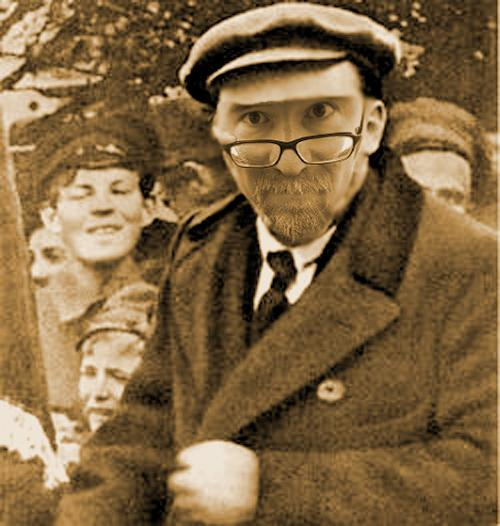
\includegraphics[height = 100pt, keepaspectratio = true]{polly}
    
    \textbf{Believe what Chairman Alroy says about \(p\)-values!}
    But you can still use ANOVA to test for difference sin means, though believe what our Beloved Chairman says about asking what is the difference, why is it, and do I believe it!
  \end{frame}
  
  
  
  \begin{frame}
    \frametitle{Take home message}
    \huge{``Significance`` is a product of interpretation, not of rigid rules.}
    \\~\\
    \huge{Statistical inference is concerned with the ``art of approximation''} \small{(Akaike)}.
  \end{frame}



  \begin{frame}
    \frametitle{Commandment 4}
    \textbf{Thou shalt worship the almighty power! }
    Despite the preceding commandment, accepting the null hypothesis is a vile, ungodly thing. 
    Always make sure thou hast the statistical power and \emph{a small enough difference relative to what thou carest about} to argue that a difference doesn't matter (not just that it isn't ``significant''). 
    When in doubt, find a power calculator on the web and do a proper power analysis.
  \end{frame}
  
  
  
  \begin{frame}
    \frametitle{Commandment 5}
    \textbf{Thou shalt abhor tiny little time series! }
    All too often people are seduced by ``trends'' of two or three data points, damning themselves to eternal hellfire. 
    The two-tailed probability of a flawless ``trend'' with six points is 0.0625 (!). 
    ``Before'' and ``after'' comparisons are no better than a single coin flip, unless the points in each category have significantly different averages. 
    Coincidences are often coincidences: if (say) the biggest extinction happened in the same interval as the biggest climate change, and there are ten intervals, well, \(p\) = 0.10. 
    So, demand that a time series analysis include a healthy number of data points, at least a dozen or a score or a cubit.
  \end{frame}



  \begin{frame}
    \frametitle{Commandment 6}
    \textbf{Thou shalt difference thy data! }
    Time series data are almost always autocorrelated (and thou shalt test for that). 
    Still, people insist on interpreting ``trends'' shared by pairs of time series as meaningful cross-correlations, even though autocorrelation makes finding these demonic things \emph{the null hypothesis!} 
    Even random walks produce such patterns! FEAR YE SINNERS! 
    The easiest and most powerful way to remove the autocorrelation is to take first differences. 
    So, the next time thou wantest to correlate population growth with the rate of sea-floor spreading - and people will - \emph{difference thy \%\!\@\#\$\% data}.
  \end{frame}



  \begin{frame}
    \frametitle{Commandment 7}
    \textbf{Thou shalt not play with PCA!} 
    Principal components analysis assumes linear responses of observed variables to underlying variables, but most ecological data show modal responses. 
    Vain mortal, what power grants thee the right to assume linearity? 
    Correspondence analysis can handle both kinds of responses and works wonderfully on modal data (we won't mention that nasty little arch effect...).
  \end{frame}
  
  
  
  \begin{frame}
    \frametitle{PCA}
    Ecological data had a lot of 0s.
    \\~\\
    Euclidean distance from data with a lot of 0's is not a fantastic thing.
    
    % example plot from my invertebrate data set
  \end{frame}
  
  
  
  \begin{frame}
    \frametitle{PCA}
    Alternatives like CA or PCoA provide huge improvements for data with lots of 0s.
    \\~\\
    No Euclidean assumption.
    \\~\\
    PCoA is very similar to PCA, CA is wildly different.
    
    % example stuff from Tom's lectures.
  \end{frame}
  
  
  
  \begin{frame}
    \frametitle{Commandment 8}
    \textbf{Thou shalt not cluster shamelessly!} 
    The world is full of fuzziness and apostasy, not cool, clean Platonic categories. 
    But cluster analysis imposes categories on data regardless of whether they're gradiential. 
    If the clusters are really there, thou shalt see them as a ray of divine light in the shadowy purgatory of a multivariate ordination space. 
    So why bother?
  \end{frame}
  
  
  
  \begin{frame}
    \frametitle{Commandment 9}
    \textbf{Thou shalt stand awe-struck before the shining brilliance of the G-test!} 
    Chi-square this, chi-square that. 
    The G is easier to compute, it doesn't blow up as easily because of small values, it depends on the awesome power of the log transform, it stands for ``GOD,'' and most importantly it's a maximum likelihood ratio...
  \end{frame}
  
  
  
  \begin{frame}
    \frametitle{}
    G-test now appears in Sokal and Rohlf's ``Biometry''
    
    Also, this makes more sense in the context of...
  \end{frame}



  \begin{frame}
    \frametitle{Commandment 10}
    \textbf{Thou shalt sing the praises of likelihood, not ``fit''!} 
    Anyone can design another fit statistic. 
    Why minimize the sum of squares instead of the sum of cubes or just the sum of differences? 
    None of this has a theoretical basis without a notion of probability, and specifically of likelihood. 
    After all, that's what the divine theologian Popper said.
  \end{frame}
  
  
  
  \begin{frame}
    \frametitle{}
    % fit versus likelihood
  \end{frame}
  
  
  
  \begin{frame}
    \frametitle{AIC...again}
    AIC is an approximation of the Kullbach-Leibler divergence.
    ``What?'' I hear you say...
    \\~\\
    \small{Incidentally, residual sum squares are a maximum likelihood estimator.}
  \end{frame}
  
  
  
  \begin{frame}
    \frametitle{K-L divergence}
  
  \end{frame}



  \begin{frame}
    \frametitle{back to AIC}
  
  \end{frame}



  \begin{frame}
    \frametitle{}
    \huge{Hallelujah!}
    \\~\\
    \small{but wait, there's more\!}
  \end{frame}
  
  
  
  \begin{frame}
    \frametitle{My attempt at a commandment}
    \textbf{Thou shalt release thy source!}
    While our ultimate goal is to be able repeat a study with a new sample, this is more than likely infeasible if not unfundable.
    Instead, focus on reproducible reseach (or analysis) using tools like {\LaTeX} along with literate programming tools like Sweave and knitr for R.
    Start a github account and release your source to the world.
    This way people can spend more time extending and improving your initial offereing than attempting to recreate it.
    By making your steps more open, you are more accountable for your work and thus a better scientist.
  \end{frame}



  \mode<all>
  {
    \usebackgroundtemplate{\centering 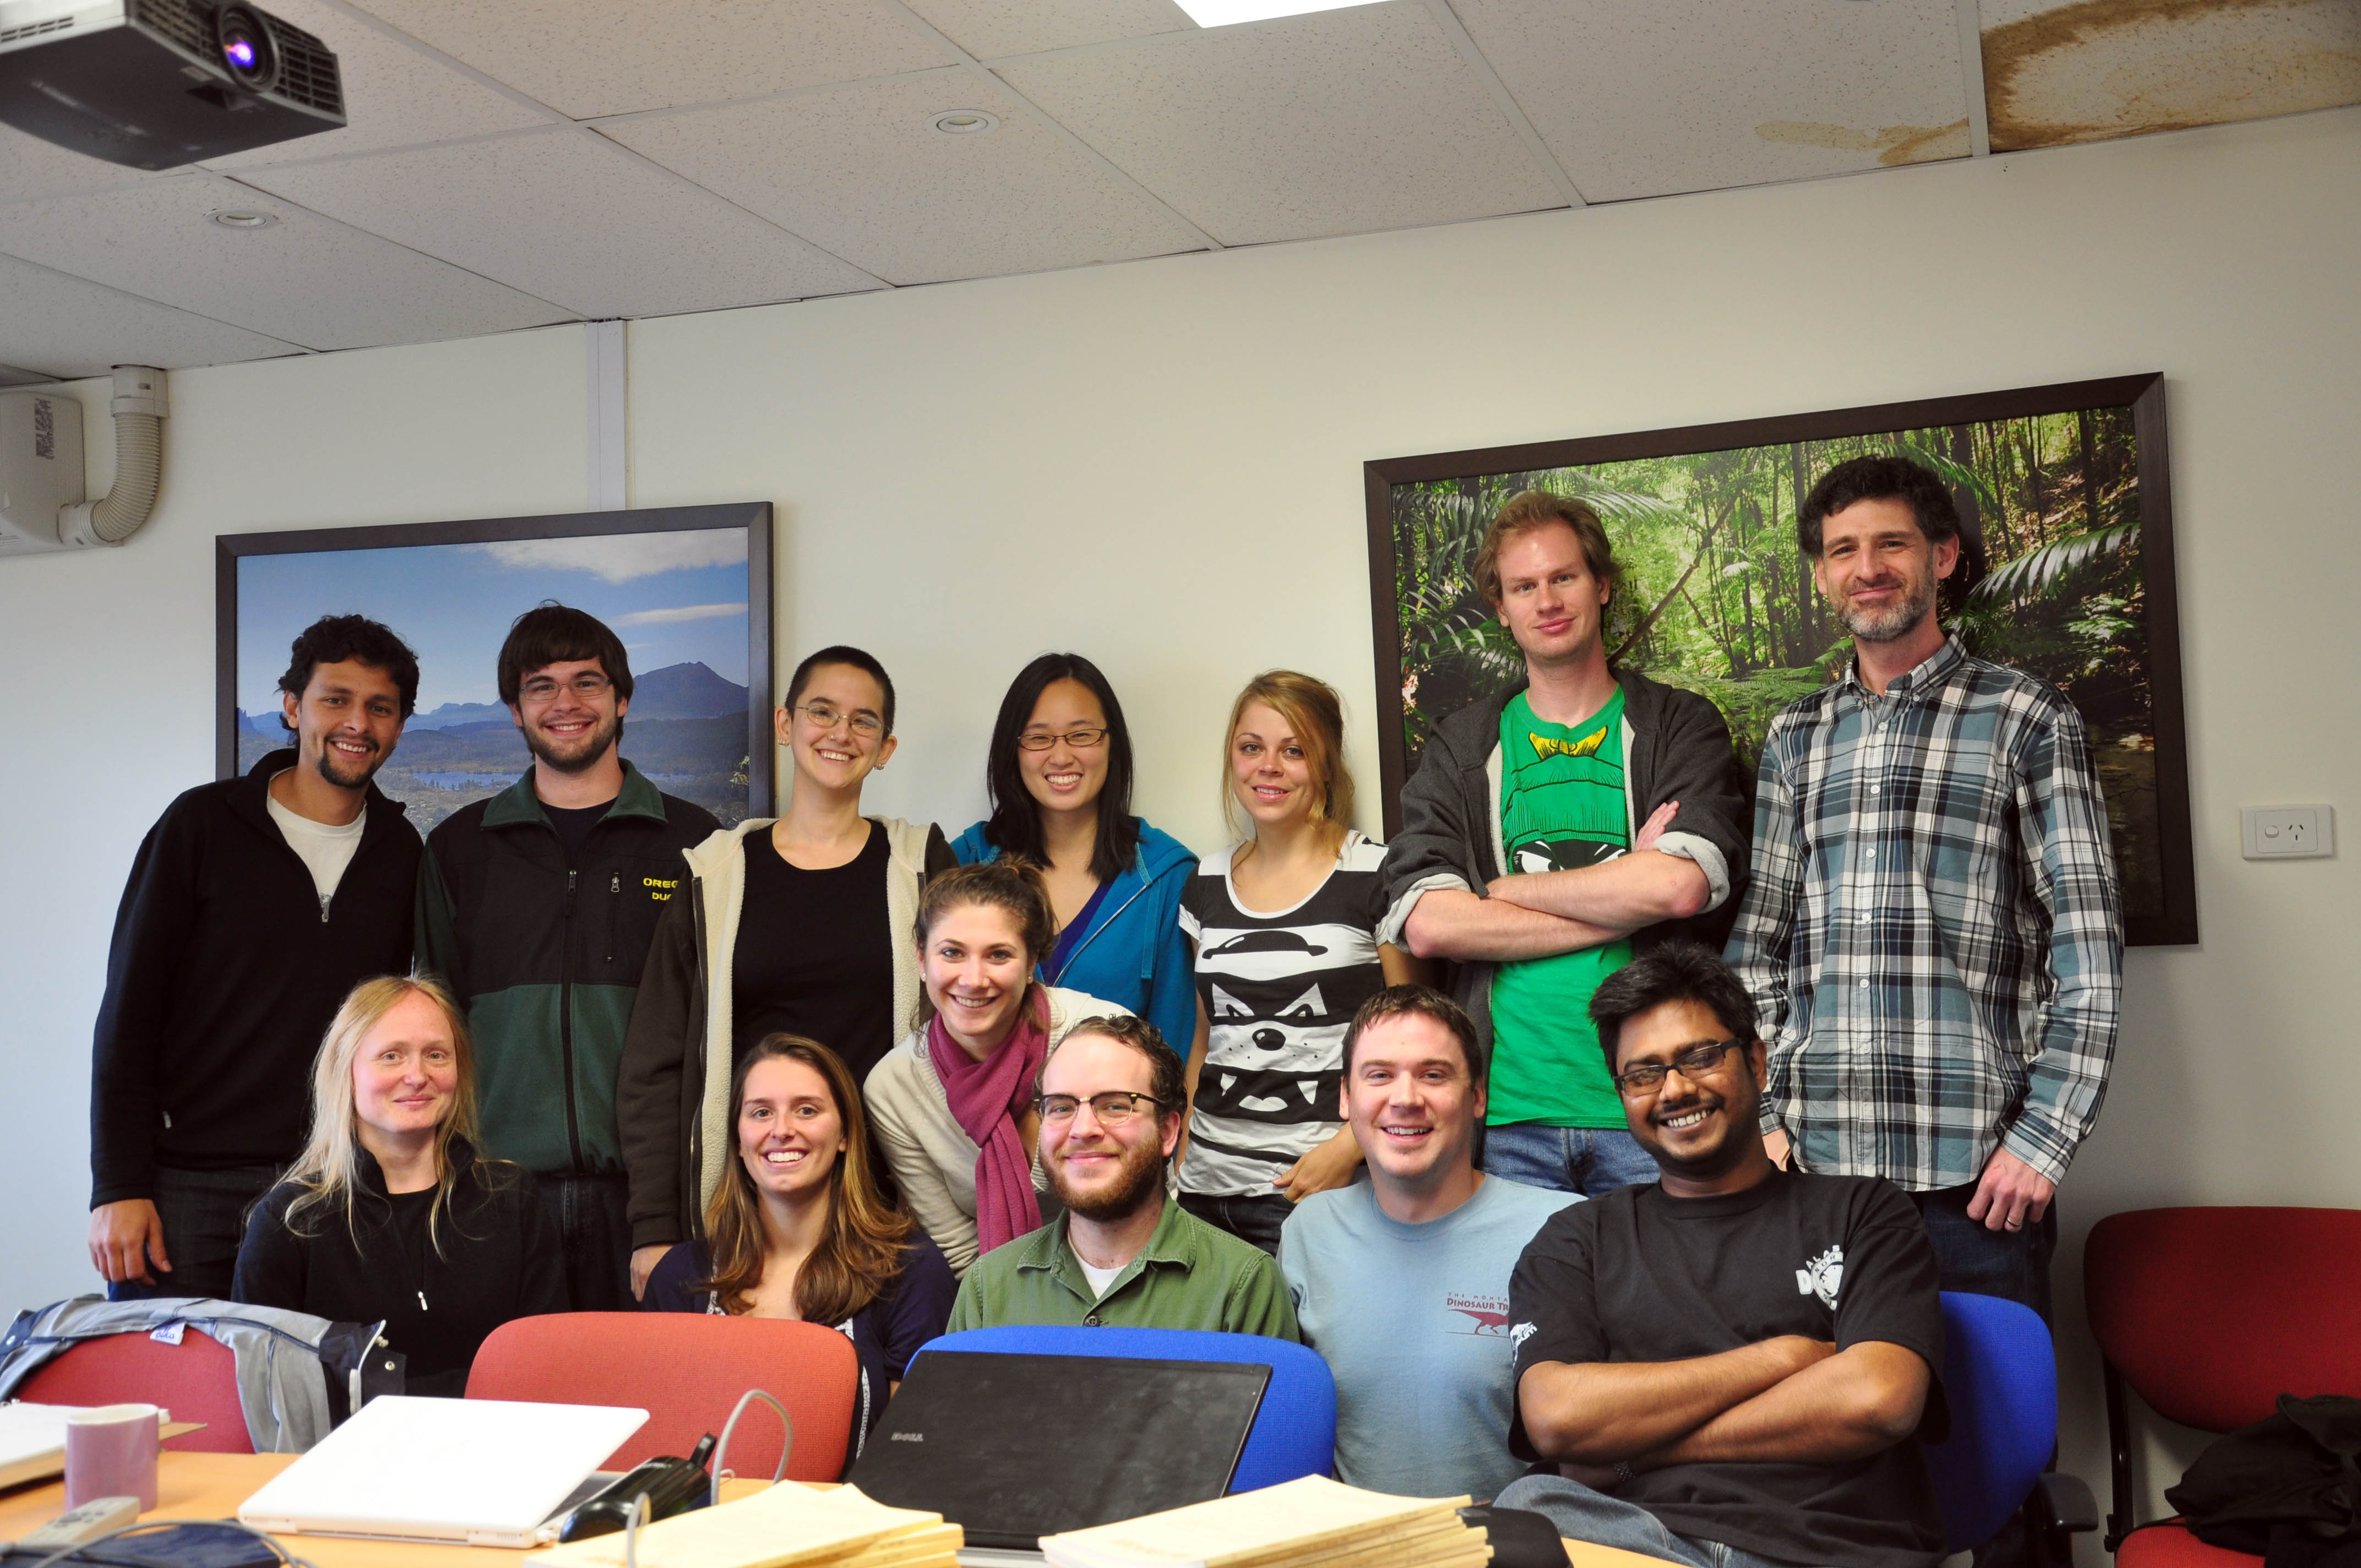
\includegraphics[width=\paperwidth]{alroy_group}}
    \begin{frame}[plain]
    \end{frame}
  }
  \mode<all>{\usebackgroundtemplate{}}
  \mode*



\end{document}
